\documentclass[russian,14pt,twoside]{extreport}
\usepackage[russian,english]{babel}
\usepackage[T2A]{fontenc}
\usepackage[utf8x]{inputenc}
\usepackage{iflang}
%%----------------------------------------------------------------------------
\usepackage{setspace}
\selectfont
\parindent=18pt
\frenchspacing
%%----------------------------------------------------------------------------
\usepackage{amsmath}
\usepackage{amssymb}
\usepackage{amscd}
\usepackage{etoolbox}
\usepackage{mathtools}
\usepackage{bm}
\usepackage[labelformat=empty]{caption}
\usepackage{graphicx}
\usepackage[all]{xy}
\usepackage{url}
\usepackage{listings}
\usepackage{array}
\usepackage{tabularx}
\usepackage{booktabs}
%%----------------------------------------------------------------------------
\usepackage[%
        a4paper,%
        includehead,%
        left=2.3cm,%    
        top=2.3cm,%
        right=2.3cm,%
        bottom=2.3cm,%
        headheight=0.7cm,%
        headsep=0.3cm,%
        footskip=1.6cm]{geometry}
\special{papersize=210mm,297mm}
%%----------------------------------------------------------------------------
\renewcommand{\thefootnote}{\fnsymbol{footnote}}
%%----------------------------------------------------------------------------
\usepackage{fancyhdr}
\pagestyle{fancy}%
\fancyhead{}%
\fancyfoot{}%
\fancyhead[LE,RO]{\normalsize \thepage}%
\fancyhead[RE,LO]{\leftmark}
%%----------------------------------------------------------------------------
\raggedbottom
%%----------------------------------------------------------------------------
\makeatletter
%%----------------------------------------------------------------------------
\protected\def\switchinitials#1{%
\begingroup%
\edef\temp{\endgroup%
    \noexpand\switchinitials@fixcomma%
    \forcsvlist{\switchinitials@item}{#1}\relax}%
    \temp}
\def\switchinitials@fixcomma, #1{#1}
\def\switchinitials@item#1{, \switchinitials@single#1\relax}
\def\switchinitials@single#1~#2\relax{#2~#1}
%%----------------------------------------------------------------------------
\newenvironment{ptkarticle}[3][russian]{%
\begin{otherlanguage}{#1}
\pagebreak[2]
\vskip 30pt plus 12pt minus 6pt
{\leftskip=1.5\parindent
\rightskip=1.5\parindent
\vbox{\centering\sffamily\bfseries\Large #2}}
\markboth{\switchinitials{#3}}{}
\nopagebreak
\vskip 6pt
\@afterheading
}{%
\end{otherlanguage}
}
%%----------------------------------------------------------------------------
\newcommand\OneAuthor[3]{%
\vbox{%
{\centering\bfseries\normalsize #1\par}
\vskip 3pt
\raggedright
\leavevmode\noindent\footnotesize
\hangindent=18pt\hangafter=1
#2, e-mail: \texttt{#3}\\*\par}
\nopagebreak
\medskip
\@afterheading
}
%%----------------------------------------------------------------------------
\newcommand\TwoAuthor[6]{%
\vbox{%
{\centering\bfseries\normalsize #1$^1$, #4$^2$\\}
\vskip 3pt
\raggedright
\leavevmode\noindent\footnotesize
\hangindent=18pt\hangafter=1
$^1$ {#2}, e-mail: \texttt{#3}\par
\hangindent=18pt\hangafter=1
$^2$ {#5}, e-mail: \texttt{#6}\\*\par}
\nopagebreak
\smallskip
\@afterheading
}
%%----------------------------------------------------------------------------
\newcommand\ThreeAuthor[9]{%
\vbox{%
{\centering\bfseries\normalsize #1$^1$, #4$^2$, #7$^3$\\}
\vskip 3pt
\raggedright
\leavevmode\noindent\footnotesize
\hangindent=18pt\hangafter=1
$^1$ {#2}, e-mail: \texttt{#3}\par
\hangindent=18pt\hangafter=1
$^2$ {#5}, e-mail: \texttt{#6}\par
\hangindent=18pt\hangafter=1
$^3$ {#8}, e-mail: \texttt{#9}\\*\par}
\nopagebreak
\smallskip
\@afterheading
}
%%----------------------------------------------------------------------------
\newcommand\FourAuthor[9]{%
\def\Argi{{#1}}%
\def\Argii{{#2}}%
\def\Argiii{{#3}}%
\def\Argiv{{#4}}%
\def\Argv{{#5}}%
\def\Argvi{{#6}}%
\def\Argvii{{#7}}%
\def\Argviii{{#8}}%
\def\Argix{{#9}}%
\FourAuthorContinue
}
\newcommand\FourAuthorContinue[3]{%
\vbox{%
{\centering
{\bfseries\normalsize \Argi$^1$, \Argiv$^2$, \Argvii$^3$, #1$^4$\\}}
\vskip 3pt
\raggedright
\leavevmode\noindent\footnotesize
\hangindent=18pt\hangafter=1
$^1$ \Argii, e-mail: \texttt{\Argiii}\par
\hangindent=18pt\hangafter=1
$^2$ \Argv, e-mail: \texttt{\Argvi}\par
\hangindent=18pt\hangafter=1
$^3$ \Argviii, e-mail: \texttt{\Argix}\par
\hangindent=18pt\hangafter=1
$^4$ #2, e-mail: \texttt{#3}\\*\par}
\nopagebreak
\smallskip
\@afterheading
}
%%----------------------------------------------------------------------------
\newcommand\FiveAuthor[9]{%
\def\Argi{{#1}}%
\def\Argii{{#2}}%
\def\Argiii{{#3}}%
\def\Argiv{{#4}}%
\def\Argv{{#5}}%
\def\Argvi{{#6}}%
\def\Argvii{{#7}}%
\def\Argviii{{#8}}%
\def\Argix{{#9}}%
\FiveAuthorContinue
}
\newcommand\FiveAuthorContinue[6]{%
\vbox{%
{\centering
\bfseries\normalsize \Argi$^1$, \Argiv$^2$, \Argvii$^3$, #1$^4$, #4$^5$\\}
\vskip 3pt
\raggedright
\leavevmode\noindent\footnotesize
\hangindent=18pt\hangafter=1
$^1$ {\Argii}, e-mail: \texttt{\Argiii}\par
\hangindent=18pt\hangafter=1
$^2$ {\Argv}, e-mail: \texttt{\Argvi}\par
\hangindent=18pt\hangafter=1
$^3$ {\Argviii}, e-mail: \texttt{\Argix}\par
\hangindent=18pt\hangafter=1
$^4$ {#2}, e-mail: \texttt{#3}\par
\hangindent=18pt\hangafter=1
$^5$ {#5}, e-mail: \texttt{#6}\\*\par}
\nopagebreak
\smallskip
\@afterheading
}
%%----------------------------------------------------------------------------
\newcommand\Subtitle[1]{
\medskip
\noindent
{\bfseries\large #1}
\par\nopagebreak
\smallskip
\@afterheading
}
%%----------------------------------------------------------------------------
\usepackage{enumitem}
\setlist[enumerate]{%
    %labelindent=0pt by default
    leftmargin=*,%
    topsep=4pt plus 2pt minus 2pt,%
    partopsep=2pt plus 1pt minus 1pt,%
    parsep=2pt plus 1pt,%
    itemsep=2pt plus 1pt%
}
\setlist[itemize]{%
    %labelindent=0pt by default
    leftmargin=*,%
    topsep=4pt plus 2pt minus 2pt,%
    partopsep=2pt plus 1pt minus 1pt,%
    parsep=2pt plus 1pt,%
    itemsep=2pt plus 1pt%
}
%%----------------------------------------------------------------------------
\newenvironment{ptkreferences}{
\pagebreak[1]
\medskip
\noindent
{\scshape\large \IfLanguageName{russian}{Список литературы}{References}}
\par\nopagebreak
\smallskip
\@afterheading
\begin{enumerate}[label={[\arabic*]},leftmargin=*]
}{
\end{enumerate}
}
%%----------------------------------------------------------------------------
\binoppenalty=10000
\relpenalty=10000
\@clubpenalty=10000
\clubpenalty=10000
\widowpenalty=10000
%%----------------------------------------------------------------------------
\defineshorthand[russian]{"*}{\mbox{-}\bbl@allowhyphens}
%%----------------------------------------------------------------------------
\makeatother
%%----------------------------------------------------------------------------
\begin{document}
% -*- Coding: cp1251; -*-

%\newcommand{\No}{\textnumero}
\begin{ptkarticle}[russian]%
{�������� �������� ���������� �������� ��������� ���������� � ������� ������ ������������ � ����������� ���������� � ����������}{���������~�.\,�., �����~�.\,�.}
\TwoAuthor%
{��������� ������ ����������}%
{������������ ����������������� ������������� ��������������� ����������� ��.~�.�.~������������}{kocheganov@gmail.com}%
{����� ������ ������������}%
{������������ ����������������� ������������� ��������������� ����������� ��.~�.�.~������������}{andrei.zorine@itmm.unn.ru}

\Subtitle{���������� ������}

� ������ ������ ��������������� ���� (������) �� ���� ������ ���������
������������. � ������ �� ��� ������������� ����������� ������ �� ������������
���������, � �� ������ "--- �� ��������� � �����������. ������ ��������� ����
�������� ������� � ������~[1]. ����������� ��� ������ �������� �����������
������ ������ ��� ������ ������� ��������� ������������. �������� ������������
������� �� �������� �������.  �� ���� �������������� ���������� ��������� ������
������� ������ ����������: $\Pi_1$, $\Pi_2$, $\Pi_3$ � $\Pi_4$.  ����������
�������� ������~$\Pi_j$ ��������� � ������� $O_j$ � �������������� ������������,
$j \in \{1,2,3,4\}$. ���������� �� ������� $O_j$ ������������� � �������
�����������. ���������� ������� �������~$\Pi_1$ �~$\Pi_3$ ����������� �������
������, ������� ����� ���� ���������. ������ �� ���� ������� ��������
������������ ������������� �������. ��������� $\lambda_1$ � $\lambda_3$
������������� ������� ����� ���������� ������� $\Pi_1$ � $\Pi_3$
��������������. ������������ ������� ���������� ���������� � ������ �� ������
$\Pi_j$ ����� ��� $f_j(z) = \sum_{\nu=1}^{\infty} p_{\nu}^{(j)} z ^{\nu}$, $j\in
\{1,3\}$.  ��������������, ��� $f_j(z)$ �������� ��� ������ $z\in \mathbb{C}$
������, ��� $|z|<\nobreak\discretionary{}{\hbox{$\mathsurround=0pt
    <$}}{}(1+\varepsilon)$, $\varepsilon>0$. ����� ������������, ���������� ��
������� $O_1$ ��������� ������� � ������� ��� ���������� ������
$\Pi_4$. ���������� ������~$\Pi_4$, � ���� �������, ����� ������������ ���������
� ������� � �������� ���������� ������ $\Pi_2$. ������ $\Pi_2$ � $\Pi_3$
����������� � ��� ������, ��� �� ���������� �� ����� ���� ���������
������������. 

����������� ������������� ����� ����� $d$, $n_0$, $n_1$, $\ldots$,
$n_d$. ����� ��������� ��������� �������������� ���������� ����� ��������� ��������� �������: $\Gamma=\{\Gamma^{(k,r)} \colon k=0,1,\ldots,d; r=1,2,\ldots
n_k\}$. � ���������  $\Gamma^{(k,r)}$ ������ ��������� � ������� ������������
�������  $T^{(k,r)}$. �������� ����� ��������� ��������� ����������
��������� �������, ��� � ����� ������� $O_3$ � ������ �������� ������� �
��������� ������ � ������~[1]. 

��� ������� �������� ������������ ������������ ������ ���������
$\Pi^{\mathrm{sat}}_1$, $\Pi^{\mathrm{sat}}_2$, $\Pi^{\mathrm{sat}}_3$,
$\Pi^{\mathrm{sat}}_4$.  ����� ���������� � ������ ���������
$\Pi^{\mathrm{\text{sat}}}_j$ �� ����� $T^{(k,r)}$ ���������� � ����� $\ell(k,r,j)$, ����
������������� ���������� ��������� � ��������� $\Gamma^{(k,r)}\in \Gamma$.

�������������� ������� ��������� ������������ ����� ��������������� ���
��������������� ����������� �������.  ����� ����������� �������
������������ �� ���.~1. �� ����� ������������ ��������� �����: ������� ����� �
����� ����������, ������� ������ (������� ������ $\Pi_1$, $\Pi_2$, $\Pi_3$,
$\Pi_4$ � ������ ��������� $\Pi^{\mathrm{sat}}_1$, $\Pi^{\mathrm{sat}}_2$, $\Pi^{\mathrm{sat}}_3$,
$\Pi^{\mathrm{sat}}_4$), ������� ������ (������� $O_1$, $O_2$, $O_3$, $O_4$), ���������� ��
����������� ������� ������ (���������� ����������� ��������� ��������
$\delta_1$, $\delta_2$, $\delta$, $\delta_4$), ���������� ������ (�������������
����������, ��), ���������� �� ����������� ���������� ������ (���� ��������� ��
������ ��������� �� � ������), �������� ������ (�������� ������
$\Pi^{\mathrm{\text{out}}}_1$, $\Pi^{\mathrm{\text{out}}}_2$,
$\Pi^{\mathrm{\text{out}}}_3$, $\Pi^{\mathrm{\text{out}}}_4$).
\sloppy 

\begin{figure}[h!]
   \centering
    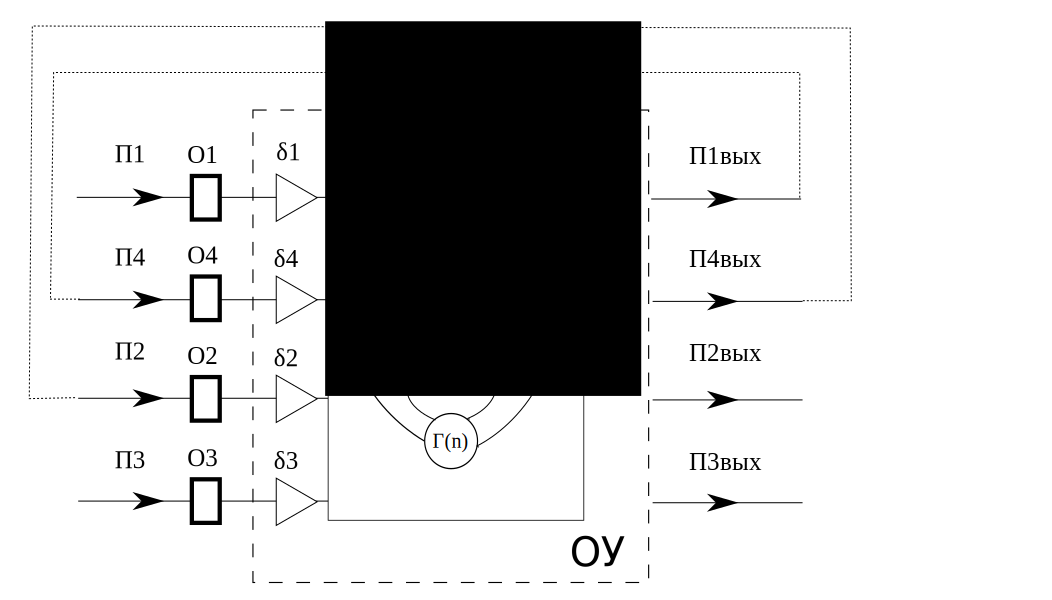
\includegraphics[width=13cm]{SystemScheme.pdf}
    \caption {���.~1: ����� ��� ��� ����������� ��������������� �������}
\end{figure}

� ������~[2] ���� �������� ����������, ���������� � ������� ������ �������. ���
��������� ������������� ������ ������������������ ��������� ������� � ���������
���������, ����������� ���������� ��������� ����� ���������� � ��������� ����
������ �����. � ���������, � �������� ���������� ��������� ����� �������
������������������ $\tau_0=0$, $\tau_1$, $\tau_2$, $\ldots$ �������� �����
��������� �������������� ����������. ��������� $\Gamma_i\in\Gamma$, $i=1$, $2$,
\ldots{} ��������� �������������� ���������� � ������� �������
$\left(\tau_{i-1};\tau_i\right]$ � $\Gamma_0\in \Gamma$ ��� ��������� � ������
������� $\tau_0$ � ����� $\varkappa_{j,i} \in \mathbb{Z}_+ $ "--- ����������
���������� � ������� $O_j$ � ������ ������� $\tau_i$, , $i\geqslant 0$.  
���� ��������, ��� �������������� ������������������ $\{(\Gamma_i,
\varkappa_{1,i}, \varkappa_{2,i}, \varkappa_{3,i}, \varkappa_{4,i}); i=0, 1,
\ldots\}$ �������� ���������� ����� �������. �������� ������������������ $\{(\Gamma_i,\varkappa_{3,i}); i \geqslant 0\}$ ������� � �������~[1,3].


\Subtitle{�������� ���������}

� ������ ������ �� ������������� ������������������  
\[
\{(\Gamma_i,
\varkappa_{1,i},\varkappa_{3,i}); i \geqslant 0\}. \tag{1} 
\]

\noindent{\bfseries ������� 1.}  {\itshape 
  �������������� ������������������~(1)
  ��� �������� ������������� �������� $(\Gamma_0, \varkappa_{1,0},
  \varkappa_{2,0}, \varkappa_{3,0}, \varkappa_{4,0})$ �������� ���������� �����
  �������.  
}

\smallskip

\noindent
{\bfseries ������� 2.}
{\itshape
��� ����, ����� ���������� ����~(1) ����� ������������ �������������,  ���������� ���������� ����������� 
$$
\min_{\substack{k=\overline{1,d}\\ j=1,3}} { \frac{\sum_{r = 1}^{n_k} \ell(k,r,j) }{\lambda_j f_j'(1) \sum_{r=1}^{n_k} T^{(k,r)} }}>1.
$$
}


\begin{ptkreferences}
\selectlanguage{english}
\item
Kocheganov~V.\,M., Zorine~A.\,V. Low-Priority Queue and Server�s Steady-State
Existence in a Tandem Under Prolongable Cyclic Service~//  Distributed Computer
and Communication Networks. DCCN 2016. Communications in Computer and
Information Science (Vishnevskiy V., Samouylov K., Kozyrev D. (eds)). ---
Springer, Cham.--- V.\,678. --- 2016. --- pp.\,210--221. 
\selectlanguage{russian}
\item
���������~�.\,�., �����~�.\,�. ������������� ������ ������� ������ ��������� ������������ � ����������� ����������� � ���������� // ������ ������������, ��������� ��������, �������������� ���������� � ����������: ��������� ��������. ����. ����., ������. 80-����� ����., �-�� ���.-���. ���� �.\,�. ���������, ����� "--- 23�26 ����. 2015. "--- �.\,94--99.

\item
Kocheganov~V.\,M., Zorine~A.\,V. Low-priority queue fluctuations in tandem of queueing systems under cyclic control with prolongations // �������������� ������������ � ��������������������� ����: ����������, ����������, ����� (DCCN-2015) : ��������� ������������� ��������. ����. ������., 19�22 ���. 2015 �., ������: / ��-� ������� ���. ��. �.�. ������������ ���. ����. ���� ; ��� ���. ���. �.�. �����������. ��.: ��� ��� "--- 2015. "--- �.~517--524.


\end{ptkreferences}

\end{ptkarticle}    

%%% Local Variables:
%%% �oding: cp1251
%%% TeX-PDF-mode: t
%%% TeX-master: "ptk18main.tex"
%%% End:

\end{document}